\documentclass{article}
\usepackage{amsmath,amssymb,amsfonts,amsthm}
\usepackage{multicol}
\usepackage{multirow}
\usepackage{mathtools}
\usepackage{soul}
\usepackage{hyperref}
\hypersetup{
    colorlinks=true,
    linkcolor=blue,
    filecolor=magenta,      
    urlcolor=cyan,
    pdftitle={Overleaf Example},
    pdfpagemode=FullScreen,
    }
\usepackage{color}
\usepackage[table]{xcolor}
\usepackage[T1]{fontenc}
\usepackage{etoolbox}
\usepackage{multicol}
\usepackage{multirow}
\usepackage{geometry}
\geometry{
    a4paper,
    left=2cm,
    right=2cm,
    top=2cm,
    bottom=2cm
}
\usepackage{fancyhdr}
\usepackage{graphicx}
\usepackage{tcolorbox}
\usepackage{array}
\usepackage{amsthm}
\usepackage{titlesec}
\usepackage{tikz, tkz-euclide}
  \usetikzlibrary{arrows.meta,calc}
  \newcommand\rightAngle[4]{
  \pgfmathanglebetweenpoints{\pgfpointanchor{#2}{center}}{\pgfpointanchor{#1}{center}}
  \coordinate (tmpRA) at ($(#2)+(\pgfmathresult+45:#4)$);
  \draw[red!60!black,thick] ($(#2)!(tmpRA)!(#1)$) -- (tmpRA) -- ($(#2)!(tmpRA)!(#3)$);
}
\renewcommand{\baselinestretch}{1.2}

\titleformat*{\section}{\large\bfseries}
\titleformat*{\subsection}{\normalsize\bfseries}

\newtheorem{theorem}{Theorem}
\newtheorem*{teorema}{Teorema}
\newtheorem*{definisi}{Definisi}
\theoremstyle{definition}
\newtheorem*{bukti}{Bukti}

\newcommand{\Arg}{\text{Arg}}
\newcommand{\R}{\mathbb{R}}
\newcommand{\C}{\mathbb{C}}
\newcommand{\N}{\mathbb{N}}
\newcommand{\Z}{\mathbb{Z}}

% \newtcolorbox{solution}[1][]{
%     colback=blue!5!white, 
%     colframe=blue!75!black,
%     fonttitle=\bfseries, 
%     colbacktitle=blue!50!black,
%     title=Solution,
%     #1
% }

\newenvironment{solution}{
  \textbf{Solution:}\\
}

\begin{document}
\fancyhead[L]{\textit{Teosofi Hidayah Agung}}
\fancyhead[R]{\textit{5002221132}}
\pagestyle{fancy}
\begin{enumerate}
    \item Determine the coefficients for $x^5 y^{13}$ and $x^9 y^9$ in the expansion of $(3x - 4y)^{18}$.\\
    \begin{solution}
    The general term in the binomial expansion of $(a + b)^n$ is given by
    \[
    (a + b)^n= \sum_{k=0}^{n} \binom{n}{k} a^{n-k} b^k
    \]
    For the expansion of $(3x - 4y)^{18}$, we have $a = 3x$, $b = -4y$, and $n = 18$.
    \\\begin{itemize}
        \item For the term $x^5 y^{13}$, we need to find $k$ such that $n-k = 5$ and $k = 13$. Thus, $k = 18 - 5 = 13$.
        \[
        \text{Coefficient} = \binom{18}{13} (3)^{18-13} (-4)^{13} = \binom{18}{5} (3)^5 (-4)^{13}
        \]
        \item For the term $x^9 y^9$, we need to find $k$ such that $n-k = 9$ and $k = 9$. Thus, $k = 18 - 9 = 9$.
        \[
        \text{Coefficient} = \binom{18}{9} (3)^{18-9} (-4)^{9} = \binom{18}{9} (3)^9 (-4)^{9}
        \]
    \end{itemize}
    \end{solution}

    \item Compute
    \[
    \sum_{k=1}^{n} \binom{n}{k} 2^{n - k}
    \]
    \\\begin{solution}
    We can use the binomial theorem, which states that
    \[
    (a + b)^n = \sum_{k=0}^{n} \binom{n}{k} a^{n-k} b^k
    \]
    Setting $a = 2$ and $b = 1$, we have
    \[
    (2 + 1)^n = \sum_{k=0}^{n} \binom{n}{k} 2^{n-k} 1^k
    \]
    This simplifies to
    \[
    \sum_{k=0}^{n} \binom{n}{k} 2^{n-k} = 3^n
    \]
    \end{solution}

    \item A bakery sells chocolate, cinnamon, and plain doughnuts and at a particular time has 6 chocolate, 6 cinnamon, and 3 plain. If a box contains 12 doughnuts, how many different options are there for a box of doughnuts?
    \\\begin{solution}
    We can use the stars and bars method to solve this problem. Let $x_1$, $x_2$, and $x_3$ represent the number of chocolate, cinnamon, and plain doughnuts in the box, respectively. We need to find the number of non-negative integer solutions to the equation
    \[
    x_1 + x_2 + x_3 = 12
    \]
    subject to the constraints $0 \leq x_1 \leq 6$, $0 \leq x_2 \leq 6$, and $0 \leq x_3 \leq 3$.

    We can edited the constraints by
    \[0\leq 6-x_1 \leq 6, \quad 0\leq 6-x_2 \leq 6, \quad 0\leq 3-x_3 \leq 3\]
    This means we can rewrite the equation as
    \[
    (6-x_1) + (6-x_2) + (3-x_3) = 15-12 \iff (6-x_1) + (6-x_2) + (3-x_3) = 3
    \]
    That equation isn't affected by the constraints, so we can use the stars and bars method to find the number of non-negative integer solutions to this equation.
    \[\binom{3+2}{2} = \binom{5}{2} = 10\]
    \end{solution}

    \item Determine the number of integer solutions of the equation
    \[
    x_1 + x_2 + x_3 + x_4 = 20
    \]
    which satisfy
    \[
    1 \leq x_1 \leq 6, \quad 0 \leq x_2 \leq 7, \quad 4 \leq x_3 \leq 8, \quad 2 \leq x_4 \leq 6
    \]
    \begin{solution}
    We can transform the variables to eliminate the lower bounds:
    \[
    y_1 = x_1 - 1, \quad y_2 = x_2, \quad y_3 = x_3 - 4, \quad y_4 = x_4 - 2
    \]
    This gives us the new equation:
    \[
    y_1 + y_2 + y_3 + y_4 = 13
    \]
    The new constraints are:
    \[
    0 \leq y_1 \leq 5, \quad 0 \leq y_2 \leq 7, \quad 0 \leq y_3 \leq 4, \quad 0 \leq y_4 \leq 4
    \]
    We can use the principle of inclusion-exclusion to count the number of solutions. First, we find the total number of non-negative integer solutions without constraints:
    \[
    \binom{13 + 4 - 1}{4 - 1} = \binom{16}{3} = 560
    \]
    Next, we subtract the cases that violate the constraints:
    \begin{itemize}
        \item For $y_1 > 5$: Let $y_1' = y_1 - 6$, then $y_1' + y_2 + y_3 + y_4 = 7$ with $0 \leq y_1'$, giving $\binom{10}{3} = 120$ solutions.
        \item For $y_2 > 7$: Let $y_2' = y_2 - 8$, then $y_1 + y_2' + y_3 + y_4 = 5$ with $0 \leq y_2'$, giving $\binom{8}{3} = 56$ solutions.
        \item For $y_3 > 4$: Let $y_3' = y_3 - 5$, then $y_1 + y_2 + y_3' + y_4 = 8$ with $0 \leq y_3'$, giving $\binom{11}{3} = 165$ solutions.
        \item For $y_4 > 4$: Let $y_4' = y_4 - 5$, then $y_1 + y_2 + y_3 + y_4' = 8$ with $0 \leq y_4'$, giving $\binom{11}{3} = 165$ solutions.
    \end{itemize}
    Now for the intersections:
    \begin{itemize}
        \item For $y_1 \geq 6$ and $y_2 \geq 8$: Let $y_1' = y_1 - 6$ and $y_2' = y_2 - 8$, then $y_1' + y_2' + y_3 + y_4 = -1$, which has no solutions.
        \item For $y_1 \geq 6$ and $y_3 \geq 5$: Let $y_1' = y_1 - 6$ and $y_3' = y_3 - 5$, then $y_1' + y_2 + y_3' + y_4 = 2$, giving $\binom{5}{3} = 10$ solutions.
        \item For $y_1 \geq 6$ and $y_4 \geq 5$: Let $y_1' = y_1 - 6$ and $y_4' = y_4 - 5$, then $y_1' + y_2 + y_3 + y_4' = 2$, giving $\binom{5}{3} = 10$ solutions.
        \item For $y_2 \geq 8$ and $y_3 \geq 5$: Let $y_2' = y_2 - 8$ and $y_3' = y_3 - 5$, then $y_1 + y_2' + y_3' + y_4 = 0$, giving $\binom{3}{3} = 1$ solution.
        \item For $y_2 \geq 8$ and $y_4 \geq 5$: Let $y_2' = y_2 - 8$ and $y_4' = y_4 - 5$, then $y_1 + y_2' + y_3 + y_4' = 0$, giving $\binom{3}{3} = 1$ solution.
        \item For $y_3 \geq 5$ and $y_4 \geq 5$: Let $y_3' = y_3 - 5$ and $y_4' = y_4 - 5$, then $y_1 + y_2 + y_3' + y_4' = 3$, giving $\binom{6}{3} = 20$ solutions.
    \end{itemize}
    And the other intersections are either impossible or yield no additional solutions.

    Now we can apply the principle of inclusion-exclusion:
    \[
    \text{Total solutions} = 560 - (120 + 56 + 165 + 165) + (0 + 10 + 10 + 1 + 1 + 20)= 560 - 506 + 42 = 96
    \]
    \end{solution}

    \item Determine the number of permutations of $\{1, 2, \ldots, 8\}$ in which exactly four integers are in their natural positions.
    \\\begin{solution}
      The idea is we can choose 4 positions from the 8 to be fixed, and then we need to derange the remaining 4 integers (i.e., arrange them such that none of them are in their original positions). The number of ways to choose 4 positions from 8 is given by $\binom{8}{4}=70$. 

      The number of derangements of $n$ objects, denoted as $D_n$, can be calculated using the formula:
      \[
      D_n = n! \sum_{i=0}^{n} \frac{(-1)^i}{i!}
      \]
      For $n = 4$, we have:
      \[
      D_4 = 4! \left( \frac{1}{0!} - \frac{1}{1!} + \frac{1}{2!} - \frac{1}{3!} + \frac{1}{4!} \right) = 24\cdot\frac{3}{8} = 9
      \]
      Therefore, the total number of permutations is $70 \cdot 9 = 630$.
    \end{solution}
    \item Determine the number of ways to place rooks on a $6 \times 6$ chessboard such that no two rooks can attack each other and none are placed on forbidden positions (marked with X):
    
    \begin{center}
    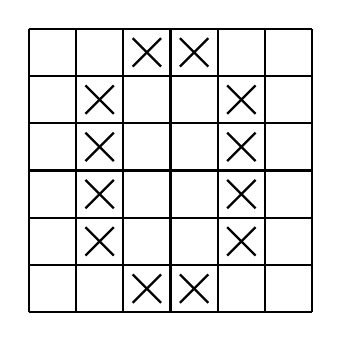
\begin{tikzpicture}[scale=0.6]
        \draw[thick] (0,0) grid (6,6);

        % Draw X marks
        \foreach \i/\j in {
            2/5, 3/5,
            4/4, 1/4,
            4/3, 1/3,
            4/2, 1/2,
            4/1, 1/1,
            2/0, 3/0
        } {
            \draw[thick] (\i+0.2,\j+0.2) -- (\i+0.8,\j+0.8);
            \draw[thick] (\i+0.8,\j+0.2) -- (\i+0.2,\j+0.8);
        }

        % Label rows and columns (optional)
        % \foreach \i in {0,...,5} {
        %     \node at (\i+0.5,6.3) {\small \i};  % column labels
        %     \node at (-0.3,5.5-\i) {\small \i};  % row labels
        % }
    \end{tikzpicture}
    \end{center}
    \begin{solution}
      Formula for the number of ways to place $k$ rooks on an $n \times n$ chessboard such that no two rooks can attack each other is given by:
      \[
      S=n!-r_1(n-1)!-r_2(n-2)!-\ldots+(-1)^k r_k(n-k)!
      \]
      where $r_i$ is the number of forbidden positions in the $i$-th row.

      Now consider the rows and columns that can be swapped. Then we can change the forbidden positions to:
      \begin{center}
      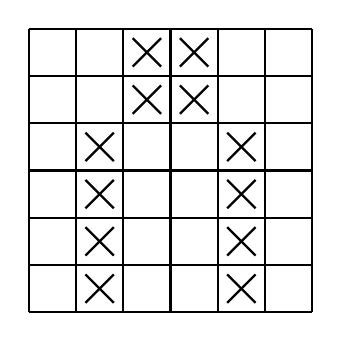
\begin{tikzpicture}[scale=0.6]
          \draw[thick] (0,0) grid (6,6);

          % Draw X marks
          \foreach \i/\j in {
              2/5, 3/5,
            4/0, 1/0,
            4/3, 1/3,
            4/2, 1/2,
            4/1, 1/1,
            2/4, 3/4
          } {
              \draw[thick] (\i+0.2,\j+0.2) -- (\i+0.8,\j+0.8);
              \draw[thick] (\i+0.8,\j+0.2) -- (\i+0.2,\j+0.8);
          }
          % Label rows and columns (optional)
          % \foreach \i in {0,...,5} {
          %     \node at (\i+0.5,6.3) {\small \i};  % column labels
          %     \node at (-0.3,5.5-\i) {\small \i};  % row labels
          % }
      \end{tikzpicture}
      \end{center}
      Then we can split by two region of forbidden positions
      \begin{center}
      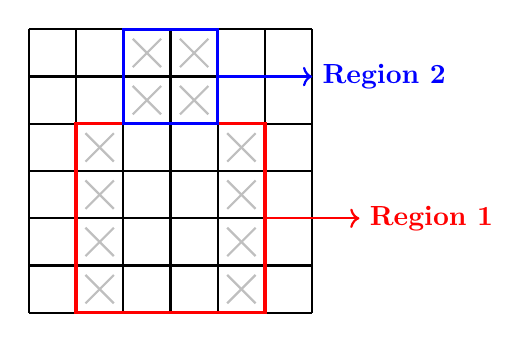
\begin{tikzpicture}[scale=0.6]
          \draw[thick] (0,0) grid (6,6);

          % Draw X marks
          \foreach \i/\j in {
              2/5, 3/5,
            4/0, 1/0,
            4/3, 1/3,
            4/2, 1/2,
            4/1, 1/1,
            2/4, 3/4
          } {
              \draw[thick,lightgray] (\i+0.2,\j+0.2) -- (\i+0.8,\j+0.8);
              \draw[thick,lightgray] (\i+0.8,\j+0.2) -- (\i+0.2,\j+0.8);
          }
          % Label rows and columns (optional)
          % \foreach \i in {0,...,5} {
          %     \node at (\i+0.5,6.3) {\small \i};  % column labels
          %     \node at (-0.3,5.5-\i) {\small \i};  % row labels
          % }
          \draw[very thick,red] (1,0) rectangle (5,4);
          \draw[->,thick,red] (5,2) -- (7,2) node[right] {\textbf{Region 1}}; 
          \draw[very thick,blue] (2,4) rectangle (4,6);
          \draw[->,thick,blue] (4,5) -- (6,5) node[right] {\textbf{Region 2}};
      \end{tikzpicture}
      \end{center}
      So we can calculate the number of ways to place rooks in each region separately.
      \begin{itemize}
        \item For one rook the possible positions such that is in forbidden positions is $r_1=12$.
        \item For two rooks the possible positions such that is in forbidden positions is $\displaystyle r_2=4\cdot 8+2+2\binom{4}{2}=34+12=46$.
        \item For three rooks the possible positions such that is in forbidden positions is $\displaystyle r_3=2\cdot 8+ 4\cdot 2\cdot\binom{4}{2}=16+48=64$.
        \item For four rooks the possible positions such that is in forbidden positions is $\displaystyle r_4=2\cdot 2\binom{4}{2}=24$.
      \end{itemize}
      For five and six rooks, there are no possible positions such that is in forbidden positions.

      Then the number of ways to place rooks on the chessboard is given by:
      \[
      S=6!-r_1(6-1)!-r_2(6-2)!-r_3(6-3)!-r_4(6-4)!=720-12\cdot 120-46\cdot 30-64\cdot 6-24\cdot 1=720-1440+1104-384+48=48
      \]
    \end{solution}
    
\end{enumerate}
\end{document}